\documentclass[1p]{elsarticle_modified}
%\bibliographystyle{elsarticle-num}

%\usepackage[colorlinks]{hyperref}
%\usepackage{abbrmath_seonhwa} %\Abb, \Ascr, \Acal ,\Abf, \Afrak
\usepackage{amsfonts}
\usepackage{amssymb}
\usepackage{amsmath}
\usepackage{amsthm}
\usepackage{scalefnt}
\usepackage{amsbsy}
\usepackage{kotex}
\usepackage{caption}
\usepackage{subfig}
\usepackage{color}
\usepackage{graphicx}
\usepackage{xcolor} %% white, black, red, green, blue, cyan, magenta, yellow
\usepackage{float}
\usepackage{setspace}
\usepackage{hyperref}

\usepackage{tikz}
\usetikzlibrary{arrows}

\usepackage{multirow}
\usepackage{array} % fixed length table
\usepackage{hhline}

%%%%%%%%%%%%%%%%%%%%%
\makeatletter
\renewcommand*\env@matrix[1][\arraystretch]{%
	\edef\arraystretch{#1}%
	\hskip -\arraycolsep
	\let\@ifnextchar\new@ifnextchar
	\array{*\c@MaxMatrixCols c}}
\makeatother %https://tex.stackexchange.com/questions/14071/how-can-i-increase-the-line-spacing-in-a-matrix
%%%%%%%%%%%%%%%

\usepackage[normalem]{ulem}

\newcommand{\msout}[1]{\ifmmode\text{\sout{\ensuremath{#1}}}\else\sout{#1}\fi}
%SOURCE: \msout is \stkout macro in https://tex.stackexchange.com/questions/20609/strikeout-in-math-mode

\newcommand{\cancel}[1]{
	\ifmmode
	{\color{red}\msout{#1}}
	\else
	{\color{red}\sout{#1}}
	\fi
}

\newcommand{\add}[1]{
	{\color{blue}\uwave{#1}}
}

\newcommand{\replace}[2]{
	\ifmmode
	{\color{red}\msout{#1}}{\color{blue}\uwave{#2}}
	\else
	{\color{red}\sout{#1}}{\color{blue}\uwave{#2}}
	\fi
}

\newcommand{\Sol}{\mathcal{S}} %segment
\newcommand{\D}{D} %diagram
\newcommand{\A}{\mathcal{A}} %arc


%%%%%%%%%%%%%%%%%%%%%%%%%%%%%5 test

\def\sl{\operatorname{\textup{SL}}(2,\Cbb)}
\def\psl{\operatorname{\textup{PSL}}(2,\Cbb)}
\def\quan{\mkern 1mu \triangleright \mkern 1mu}

\theoremstyle{definition}
\newtheorem{thm}{Theorem}[section]
\newtheorem{prop}[thm]{Proposition}
\newtheorem{lem}[thm]{Lemma}
\newtheorem{ques}[thm]{Question}
\newtheorem{cor}[thm]{Corollary}
\newtheorem{defn}[thm]{Definition}
\newtheorem{exam}[thm]{Example}
\newtheorem{rmk}[thm]{Remark}
\newtheorem{alg}[thm]{Algorithm}

\newcommand{\I}{\sqrt{-1}}
\begin{document}

%\begin{frontmatter}
%
%\title{Boundary parabolic representations of knots up to 8 crossings}
%
%%% Group authors per affiliation:
%\author{Yunhi Cho} 
%\address{Department of Mathematics, University of Seoul, Seoul, Korea}
%\ead{yhcho@uos.ac.kr}
%
%
%\author{Seonhwa Kim} %\fnref{s_kim}}
%\address{Center for Geometry and Physics, Institute for Basic Science, Pohang, 37673, Korea}
%\ead{ryeona17@ibs.re.kr}
%
%\author{Hyuk Kim}
%\address{Department of Mathematical Sciences, Seoul National University, Seoul 08826, Korea}
%\ead{hyukkim@snu.ac.kr}
%
%\author{Seokbeom Yoon}
%\address{Department of Mathematical Sciences, Seoul National University, Seoul, 08826,  Korea}
%\ead{sbyoon15@snu.ac.kr}
%
%\begin{abstract}
%We find all boundary parabolic representation of knots up to 8 crossings.
%
%\end{abstract}
%\begin{keyword}
%    \MSC[2010] 57M25 
%\end{keyword}
%
%\end{frontmatter}

%\linenumbers
%\tableofcontents
%
\newcommand\colored[1]{\textcolor{white}{\rule[-0.35ex]{0.8em}{1.4ex}}\kern-0.8em\color{red} #1}%
%\newcommand\colored[1]{\textcolor{white}{ #1}\kern-2.17ex	\textcolor{white}{ #1}\kern-1.81ex	\textcolor{white}{ #1}\kern-2.15ex\color{red}#1	}

{\Large $\underline{12a_{0448}~(K12a_{0448})}$}

\setlength{\tabcolsep}{10pt}
\renewcommand{\arraystretch}{1.6}
\vspace{1cm}\begin{tabular}{m{100pt}>{\centering\arraybackslash}m{274pt}}
\multirow{5}{120pt}{
	\centering
	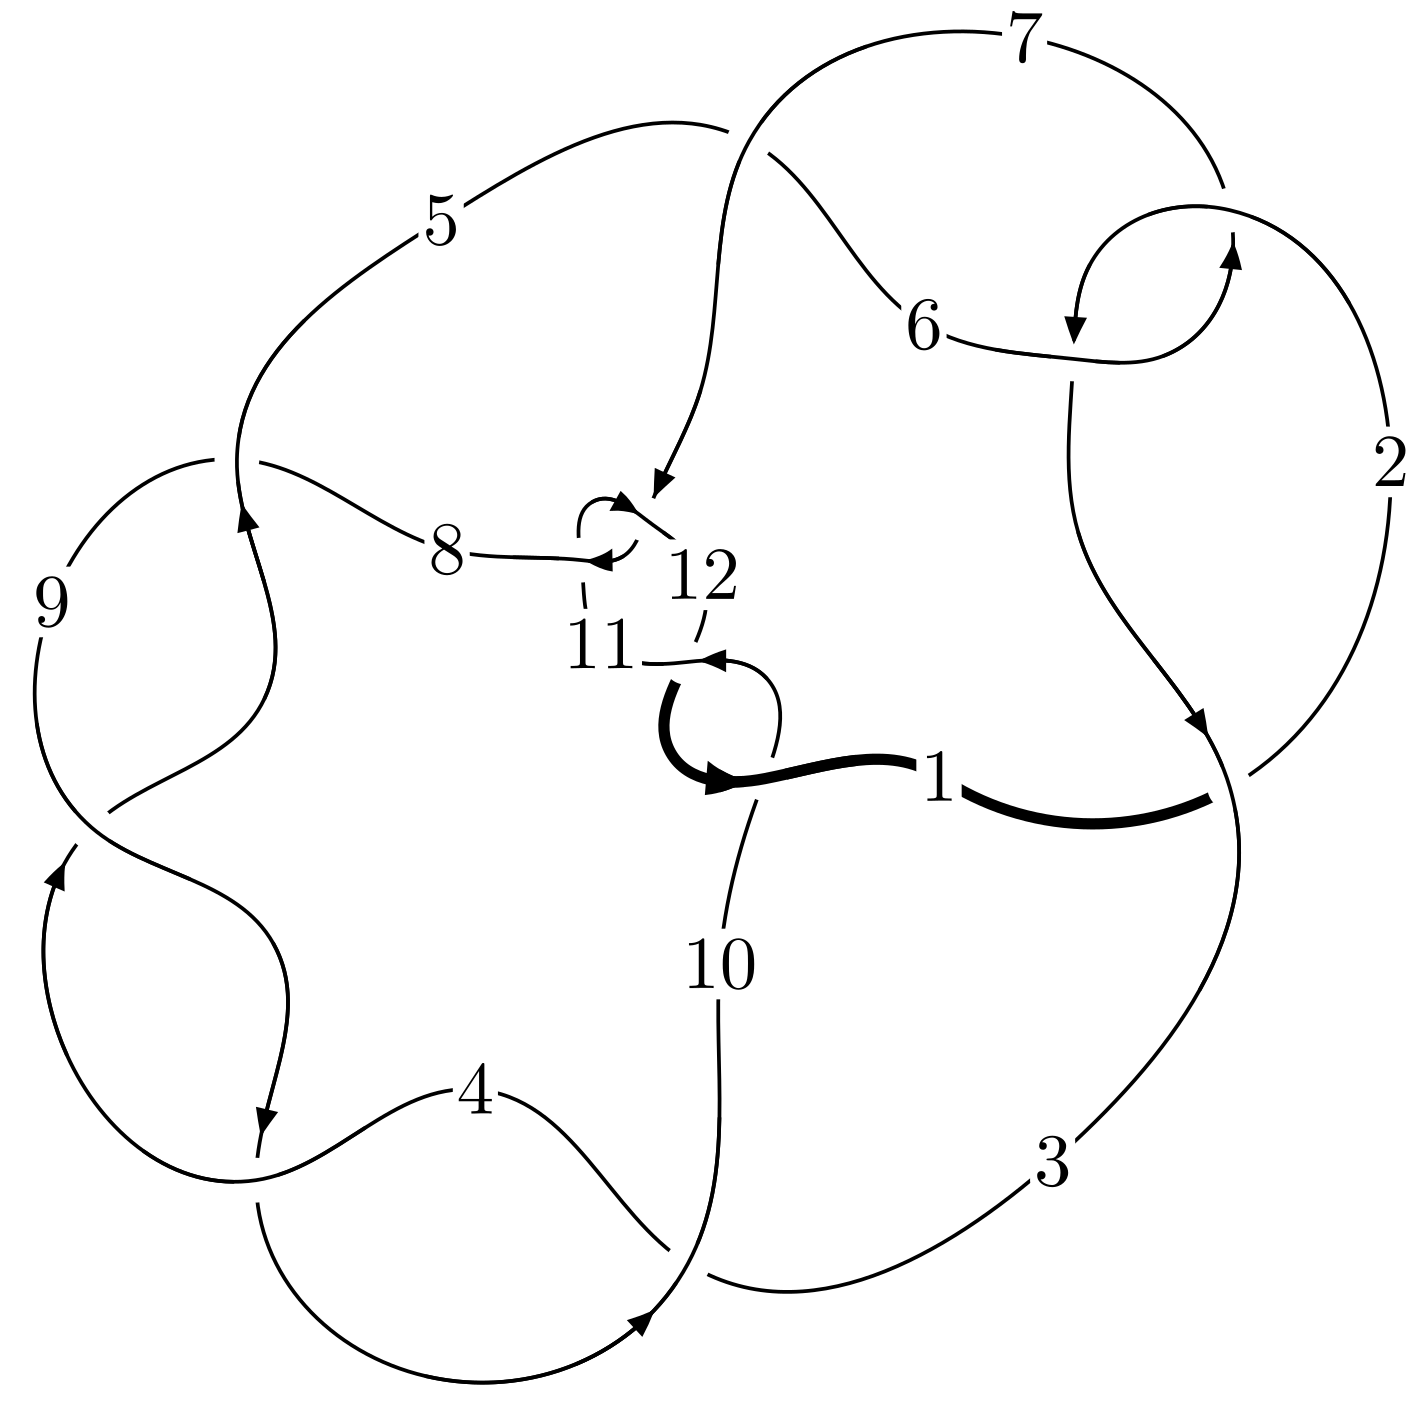
\includegraphics[width=112pt]{../../../GIT/diagram.site/Diagrams/png/1249_12a_0448.png}\\
\ \ \ A knot diagram\footnotemark}&
\allowdisplaybreaks
\textbf{Linearized knot diagam} \\
\cline{2-2}
 &
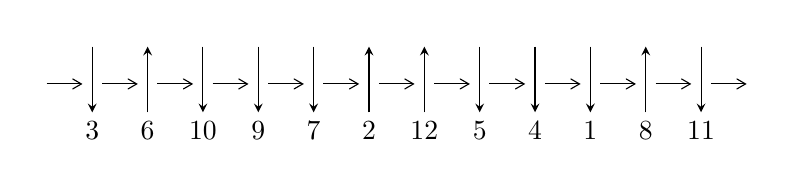
\begin{tikzpicture}[x=20pt, y=17pt]
	% nodes
	\node (C0) at (0, 0) {};
	\node (C1) at (1, 0) {};
	\node (C1U) at (1, +1) {};
	\node (C1D) at (1, -1) {3};

	\node (C2) at (2, 0) {};
	\node (C2U) at (2, +1) {};
	\node (C2D) at (2, -1) {6};

	\node (C3) at (3, 0) {};
	\node (C3U) at (3, +1) {};
	\node (C3D) at (3, -1) {10};

	\node (C4) at (4, 0) {};
	\node (C4U) at (4, +1) {};
	\node (C4D) at (4, -1) {9};

	\node (C5) at (5, 0) {};
	\node (C5U) at (5, +1) {};
	\node (C5D) at (5, -1) {7};

	\node (C6) at (6, 0) {};
	\node (C6U) at (6, +1) {};
	\node (C6D) at (6, -1) {2};

	\node (C7) at (7, 0) {};
	\node (C7U) at (7, +1) {};
	\node (C7D) at (7, -1) {12};

	\node (C8) at (8, 0) {};
	\node (C8U) at (8, +1) {};
	\node (C8D) at (8, -1) {5};

	\node (C9) at (9, 0) {};
	\node (C9U) at (9, +1) {};
	\node (C9D) at (9, -1) {4};

	\node (C10) at (10, 0) {};
	\node (C10U) at (10, +1) {};
	\node (C10D) at (10, -1) {1};

	\node (C11) at (11, 0) {};
	\node (C11U) at (11, +1) {};
	\node (C11D) at (11, -1) {8};

	\node (C12) at (12, 0) {};
	\node (C12U) at (12, +1) {};
	\node (C12D) at (12, -1) {11};
	\node (C13) at (13, 0) {};

	% arrows
	\draw[->,>={angle 60}]
	(C0) edge (C1) (C1) edge (C2) (C2) edge (C3) (C3) edge (C4) (C4) edge (C5) (C5) edge (C6) (C6) edge (C7) (C7) edge (C8) (C8) edge (C9) (C9) edge (C10) (C10) edge (C11) (C11) edge (C12) (C12) edge (C13) ;	\draw[->,>=stealth]
	(C1U) edge (C1D) (C2D) edge (C2U) (C3U) edge (C3D) (C4U) edge (C4D) (C5U) edge (C5D) (C6D) edge (C6U) (C7D) edge (C7U) (C8U) edge (C8D) (C9U) edge (C9D) (C10U) edge (C10D) (C11D) edge (C11U) (C12U) edge (C12D) ;
	\end{tikzpicture} \\
\hhline{~~} \\& 
\textbf{Solving Sequence} \\ \cline{2-2} 
 &
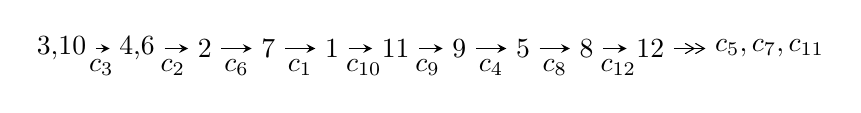
\begin{tikzpicture}[x=23pt, y=7pt]
	% node
	\node (A0) at (-1/8, 0) {3,10};
	\node (A1) at (17/16, 0) {4,6};
	\node (A2) at (17/8, 0) {2};
	\node (A3) at (25/8, 0) {7};
	\node (A4) at (33/8, 0) {1};
	\node (A5) at (41/8, 0) {11};
	\node (A6) at (49/8, 0) {9};
	\node (A7) at (57/8, 0) {5};
	\node (A8) at (65/8, 0) {8};
	\node (A9) at (73/8, 0) {12};
	\node (C1) at (1/2, -1) {$c_{3}$};
	\node (C2) at (13/8, -1) {$c_{2}$};
	\node (C3) at (21/8, -1) {$c_{6}$};
	\node (C4) at (29/8, -1) {$c_{1}$};
	\node (C5) at (37/8, -1) {$c_{10}$};
	\node (C6) at (45/8, -1) {$c_{9}$};
	\node (C7) at (53/8, -1) {$c_{4}$};
	\node (C8) at (61/8, -1) {$c_{8}$};
	\node (C9) at (69/8, -1) {$c_{12}$};
	\node (A10) at (11, 0) {$c_{5},c_{7},c_{11}$};

	% edge
	\draw[->,>=stealth]	
	(A0) edge (A1) (A1) edge (A2) (A2) edge (A3) (A3) edge (A4) (A4) edge (A5) (A5) edge (A6) (A6) edge (A7) (A7) edge (A8) (A8) edge (A9) ;
	\draw[->>,>={angle 60}]	
	(A9) edge (A10);
\end{tikzpicture} \\ 

\end{tabular} \\

\footnotetext{
The image of knot diagram is generated by the software ``\textbf{Draw programme}" developed by Andrew Bartholomew(\url{http://www.layer8.co.uk/maths/draw/index.htm\#Running-draw}), where we modified some parts for our purpose(\url{https://github.com/CATsTAILs/LinksPainter}).
}\phantom \\ \newline 
\centering \textbf{Ideals for irreducible components\footnotemark of $X_{\text{par}}$} 
 
\begin{align*}
I^u_{1}&=\langle 
- u^{17}+5 u^{16}+\cdots+4 b+8,\;-2 u^{17}+9 u^{16}+\cdots+4 a+4,\;u^{18}-5 u^{17}+\cdots-16 u+4\rangle \\
I^u_{2}&=\langle 
- u^{22} a+2 u^{22}+\cdots-4 a+5,\;- u^{22} a+u^{22}+\cdots-4 a+6,\;u^{23}+2 u^{22}+\cdots+4 u+2\rangle \\
I^u_{3}&=\langle 
- a u+b- u,\;2 a^2+a u+4 a+u+1,\;u^2+2\rangle \\
I^u_{4}&=\langle 
b^2- b+1,\;2 a- u+2,\;u^2+2\rangle \\
\\
I^v_{1}&=\langle 
a,\;b^2+b+1,\;v+1\rangle \\
I^v_{2}&=\langle 
a,\;b- v+1,\;v^2- v+1\rangle \\
\end{align*}
\raggedright * 6 irreducible components of $\dim_{\mathbb{C}}=0$, with total 76 representations.\\
\footnotetext{All coefficients of polynomials are rational numbers. But the coefficients are sometimes approximated in decimal forms when there is not enough margin.}
\newpage
\renewcommand{\arraystretch}{1}
\centering \section*{I. $I^u_{1}= \langle - u^{17}+5 u^{16}+\cdots+4 b+8,\;-2 u^{17}+9 u^{16}+\cdots+4 a+4,\;u^{18}-5 u^{17}+\cdots-16 u+4 \rangle$}
\flushleft \textbf{(i) Arc colorings}\\
\begin{tabular}{m{7pt} m{180pt} m{7pt} m{180pt} }
\flushright $a_{3}=$&$\begin{pmatrix}1\\0\end{pmatrix}$ \\
\flushright $a_{10}=$&$\begin{pmatrix}0\\u\end{pmatrix}$ \\
\flushright $a_{4}=$&$\begin{pmatrix}1\\u^2\end{pmatrix}$ \\
\flushright $a_{6}=$&$\begin{pmatrix}\frac{1}{2} u^{17}-\frac{9}{4} u^{16}+\cdots+7 u-1\\\frac{1}{4} u^{17}-\frac{5}{4} u^{16}+\cdots+6 u-2\end{pmatrix}$ \\
\flushright $a_{2}=$&$\begin{pmatrix}-\frac{1}{4} u^{16}+\frac{5}{4} u^{15}+\cdots+5 u-2\\\frac{1}{4} u^{17}-\frac{3}{4} u^{16}+\cdots+u-1\end{pmatrix}$ \\
\flushright $a_{7}=$&$\begin{pmatrix}-\frac{1}{4} u^{17}+u^{16}+\cdots+u^3+\frac{5}{2} u^2\\-\frac{1}{4} u^{17}+\frac{5}{4} u^{16}+\cdots-8 u+3\end{pmatrix}$ \\
\flushright $a_{1}=$&$\begin{pmatrix}\frac{1}{4} u^{17}- u^{16}+\cdots+6 u-3\\\frac{1}{4} u^{17}-\frac{3}{4} u^{16}+\cdots+u-1\end{pmatrix}$ \\
\flushright $a_{11}=$&$\begin{pmatrix}-\frac{1}{4} u^{16}+\frac{3}{4} u^{15}+\cdots+2 u-1\\-\frac{1}{4} u^{17}+\frac{3}{4} u^{16}+\cdots-\frac{7}{2} u^3+2 u^2\end{pmatrix}$ \\
\flushright $a_{9}=$&$\begin{pmatrix}u\\u^3+u\end{pmatrix}$ \\
\flushright $a_{5}=$&$\begin{pmatrix}u^2+1\\u^4+2 u^2\end{pmatrix}$ \\
\flushright $a_{8}=$&$\begin{pmatrix}u^3+2 u\\u^5+3 u^3+u\end{pmatrix}$ \\
\flushright $a_{12}=$&$\begin{pmatrix}-\frac{3}{4} u^{16}+\frac{9}{4} u^{15}+\cdots+6 u-3\\-\frac{5}{4} u^{17}+\frac{17}{4} u^{16}+\cdots-6 u+1\end{pmatrix}$\\&\end{tabular}
\flushleft \textbf{(ii) Obstruction class $= -1$}\\~\\
\flushleft \textbf{(iii) Cusp Shapes $= -2 u^{17}+5 u^{16}-25 u^{15}+46 u^{14}-111 u^{13}+143 u^{12}-191 u^{11}+117 u^{10}+13 u^9-240 u^8+433 u^7-502 u^6+435 u^5-247 u^4+94 u^3-14 u^2+10 u-14$}\\~\\
\newpage\renewcommand{\arraystretch}{1}
\flushleft \textbf{(iv) u-Polynomials at the component}\newline \\
\begin{tabular}{m{50pt}|m{274pt}}
Crossings & \hspace{64pt}u-Polynomials at each crossing \\
\hline $$\begin{aligned}c_{1},c_{5},c_{10}\\c_{12}\end{aligned}$$&$\begin{aligned}
&u^{18}+5 u^{17}+\cdots+9 u+1
\end{aligned}$\\
\hline $$\begin{aligned}c_{2},c_{6},c_{7}\\c_{11}\end{aligned}$$&$\begin{aligned}
&u^{18}- u^{17}+\cdots- u+1
\end{aligned}$\\
\hline $$\begin{aligned}c_{3},c_{4},c_{8}\\c_{9}\end{aligned}$$&$\begin{aligned}
&u^{18}-5 u^{17}+\cdots-16 u+4
\end{aligned}$\\
\hline
\end{tabular}\\~\\
\newpage\renewcommand{\arraystretch}{1}
\flushleft \textbf{(v) Riley Polynomials at the component}\newline \\
\begin{tabular}{m{50pt}|m{274pt}}
Crossings & \hspace{64pt}Riley Polynomials at each crossing \\
\hline $$\begin{aligned}c_{1},c_{5},c_{10}\\c_{12}\end{aligned}$$&$\begin{aligned}
&y^{18}+21 y^{17}+\cdots+25 y+1
\end{aligned}$\\
\hline $$\begin{aligned}c_{2},c_{6},c_{7}\\c_{11}\end{aligned}$$&$\begin{aligned}
&y^{18}+5 y^{17}+\cdots+9 y+1
\end{aligned}$\\
\hline $$\begin{aligned}c_{3},c_{4},c_{8}\\c_{9}\end{aligned}$$&$\begin{aligned}
&y^{18}+21 y^{17}+\cdots+64 y+16
\end{aligned}$\\
\hline
\end{tabular}\\~\\
\newpage\flushleft \textbf{(vi) Complex Volumes and Cusp Shapes}
$$\begin{array}{c|c|c}  
\text{Solutions to }I^u_{1}& \I (\text{vol} + \sqrt{-1}CS) & \text{Cusp shape}\\
 \hline 
\begin{aligned}
u &= \phantom{-}0.638269 + 0.881512 I \\
a &= -1.60019 - 0.74448 I \\
b &= \phantom{-}0.798989 - 0.998980 I\end{aligned}
 & \phantom{-}7.85728 - 11.04010 I & \phantom{-}0.91859 + 8.54564 I \\ \hline\begin{aligned}
u &= \phantom{-}0.638269 - 0.881512 I \\
a &= -1.60019 + 0.74448 I \\
b &= \phantom{-}0.798989 + 0.998980 I\end{aligned}
 & \phantom{-}7.85728 + 11.04010 I & \phantom{-}0.91859 - 8.54564 I \\ \hline\begin{aligned}
u &= \phantom{-}0.852606 + 0.090205 I \\
a &= \phantom{-}0.296474 - 0.662577 I \\
b &= -0.806782 - 0.920581 I\end{aligned}
 & \phantom{-}5.47619 + 6.09265 I & -0.58572 - 4.92211 I \\ \hline\begin{aligned}
u &= \phantom{-}0.852606 - 0.090205 I \\
a &= \phantom{-}0.296474 + 0.662577 I \\
b &= -0.806782 + 0.920581 I\end{aligned}
 & \phantom{-}5.47619 - 6.09265 I & -0.58572 + 4.92211 I \\ \hline\begin{aligned}
u &= \phantom{-}0.535129 + 1.029760 I \\
a &= -0.479909 - 0.577813 I \\
b &= \phantom{-}0.859278 + 0.833662 I\end{aligned}
 & \phantom{-}8.92136 + 1.41173 I & \phantom{-}3.03885 - 1.48819 I \\ \hline\begin{aligned}
u &= \phantom{-}0.535129 - 1.029760 I \\
a &= -0.479909 + 0.577813 I \\
b &= \phantom{-}0.859278 - 0.833662 I\end{aligned}
 & \phantom{-}8.92136 - 1.41173 I & \phantom{-}3.03885 + 1.48819 I \\ \hline\begin{aligned}
u &= \phantom{-}0.451443 + 0.440431 I \\
a &= \phantom{-}1.09739 + 1.26550 I \\
b &= -0.064887 + 0.931862 I\end{aligned}
 & -3.52462 - 1.59054 I & -11.07724 + 4.91257 I \\ \hline\begin{aligned}
u &= \phantom{-}0.451443 - 0.440431 I \\
a &= \phantom{-}1.09739 - 1.26550 I \\
b &= -0.064887 - 0.931862 I\end{aligned}
 & -3.52462 + 1.59054 I & -11.07724 - 4.91257 I \\ \hline\begin{aligned}
u &= -0.10451 + 1.44331 I \\
a &= -1.113270 + 0.030081 I \\
b &= \phantom{-}0.523980 + 0.536010 I\end{aligned}
 & \phantom{-}5.86276 + 2.35783 I & \phantom{-}3.62999 - 2.31324 I \\ \hline\begin{aligned}
u &= -0.10451 - 1.44331 I \\
a &= -1.113270 - 0.030081 I \\
b &= \phantom{-}0.523980 - 0.536010 I\end{aligned}
 & \phantom{-}5.86276 - 2.35783 I & \phantom{-}3.62999 + 2.31324 I\\
 \hline 
 \end{array}$$\newpage$$\begin{array}{c|c|c}  
\text{Solutions to }I^u_{1}& \I (\text{vol} + \sqrt{-1}CS) & \text{Cusp shape}\\
 \hline 
\begin{aligned}
u &= \phantom{-}0.08738 + 1.48686 I \\
a &= -1.038310 - 0.257211 I \\
b &= \phantom{-}0.200297 - 0.935744 I\end{aligned}
 & \phantom{-}2.79590 - 3.37304 I & -6.91564 + 4.05499 I \\ \hline\begin{aligned}
u &= \phantom{-}0.08738 - 1.48686 I \\
a &= -1.038310 + 0.257211 I \\
b &= \phantom{-}0.200297 + 0.935744 I\end{aligned}
 & \phantom{-}2.79590 + 3.37304 I & -6.91564 - 4.05499 I \\ \hline\begin{aligned}
u &= -0.285768 + 0.364542 I \\
a &= \phantom{-}0.901755 - 0.405570 I \\
b &= -0.242963 - 0.416893 I\end{aligned}
 & -0.074410 + 0.940749 I & -1.49251 - 7.14224 I \\ \hline\begin{aligned}
u &= -0.285768 - 0.364542 I \\
a &= \phantom{-}0.901755 + 0.405570 I \\
b &= -0.242963 + 0.416893 I\end{aligned}
 & -0.074410 - 0.940749 I & -1.49251 + 7.14224 I \\ \hline\begin{aligned}
u &= \phantom{-}0.19312 + 1.68324 I \\
a &= \phantom{-}1.82710 + 0.07303 I \\
b &= -0.804956 + 1.067950 I\end{aligned}
 & \phantom{-}16.6140 - 14.3108 I & \phantom{-}2.04409 + 7.60234 I \\ \hline\begin{aligned}
u &= \phantom{-}0.19312 - 1.68324 I \\
a &= \phantom{-}1.82710 - 0.07303 I \\
b &= -0.804956 - 1.067950 I\end{aligned}
 & \phantom{-}16.6140 + 14.3108 I & \phantom{-}2.04409 - 7.60234 I \\ \hline\begin{aligned}
u &= \phantom{-}0.13233 + 1.72622 I \\
a &= \phantom{-}1.108960 + 0.785050 I \\
b &= -0.962956 - 0.771207 I\end{aligned}
 & \phantom{-}18.5790 - 1.2471 I & \phantom{-}4.43961 - 1.42871 I \\ \hline\begin{aligned}
u &= \phantom{-}0.13233 - 1.72622 I \\
a &= \phantom{-}1.108960 - 0.785050 I \\
b &= -0.962956 + 0.771207 I\end{aligned}
 & \phantom{-}18.5790 + 1.2471 I & \phantom{-}4.43961 + 1.42871 I\\
 \hline 
 \end{array}$$\newpage\newpage\renewcommand{\arraystretch}{1}
\centering \section*{II. $I^u_{2}= \langle - u^{22} a+2 u^{22}+\cdots-4 a+5,\;- u^{22} a+u^{22}+\cdots-4 a+6,\;u^{23}+2 u^{22}+\cdots+4 u+2 \rangle$}
\flushleft \textbf{(i) Arc colorings}\\
\begin{tabular}{m{7pt} m{180pt} m{7pt} m{180pt} }
\flushright $a_{3}=$&$\begin{pmatrix}1\\0\end{pmatrix}$ \\
\flushright $a_{10}=$&$\begin{pmatrix}0\\u\end{pmatrix}$ \\
\flushright $a_{4}=$&$\begin{pmatrix}1\\u^2\end{pmatrix}$ \\
\flushright $a_{6}=$&$\begin{pmatrix}a\\\frac{1}{6} u^{22} a-\frac{1}{3} u^{22}+\cdots+\frac{2}{3} a-\frac{5}{6}\end{pmatrix}$ \\
\flushright $a_{2}=$&$\begin{pmatrix}-\frac{2}{3} u^{22} a+\frac{1}{12} u^{22}+\cdots-\frac{1}{6} a+\frac{5}{6}\\\frac{1}{3} u^{22} a+\frac{1}{3} u^{22}+\cdots-\frac{2}{3} a-\frac{1}{6}\end{pmatrix}$ \\
\flushright $a_{7}=$&$\begin{pmatrix}-\frac{1}{6} u^{22} a+\frac{1}{12} u^{22}+\cdots+\frac{5}{6} a+\frac{4}{3}\\\frac{1}{3} u^{22} a-\frac{1}{6} u^{22}+\cdots+\frac{1}{3} a-\frac{1}{6}\end{pmatrix}$ \\
\flushright $a_{1}=$&$\begin{pmatrix}-\frac{1}{3} u^{22} a+\frac{5}{12} u^{22}+\cdots-\frac{5}{6} a+\frac{2}{3}\\\frac{1}{3} u^{22} a+\frac{1}{3} u^{22}+\cdots-\frac{2}{3} a-\frac{1}{6}\end{pmatrix}$ \\
\flushright $a_{11}=$&$\begin{pmatrix}-\frac{1}{6} u^{22} a+\frac{1}{12} u^{22}+\cdots-\frac{7}{6} a+\frac{1}{3}\\-\frac{1}{2} u^{19}- u^{18}+\cdots+2 u^3-1\end{pmatrix}$ \\
\flushright $a_{9}=$&$\begin{pmatrix}u\\u^3+u\end{pmatrix}$ \\
\flushright $a_{5}=$&$\begin{pmatrix}u^2+1\\u^4+2 u^2\end{pmatrix}$ \\
\flushright $a_{8}=$&$\begin{pmatrix}u^3+2 u\\u^5+3 u^3+u\end{pmatrix}$ \\
\flushright $a_{12}=$&$\begin{pmatrix}-\frac{1}{6} u^{22} a+\frac{1}{12} u^{22}+\cdots-\frac{7}{6} a+\frac{4}{3}\\\frac{1}{6} u^{22} a+\frac{1}{6} u^{22}+\cdots-\frac{1}{3} a-\frac{4}{3}\end{pmatrix}$\\&\end{tabular}
\flushleft \textbf{(ii) Obstruction class $= -1$}\\~\\
\flushleft \textbf{(iii) Cusp Shapes $= - u^{22}-2 u^{21}-17 u^{20}-30 u^{19}-123 u^{18}-188 u^{17}-490 u^{16}-634 u^{15}-1160 u^{14}-1234 u^{13}-1637 u^{12}-1380 u^{11}-1295 u^{10}-836 u^9-474 u^8-258 u^7-17 u^6-62 u^5+31 u^4-24 u^3- u^2-10 u-4$}\\~\\
\newpage\renewcommand{\arraystretch}{1}
\flushleft \textbf{(iv) u-Polynomials at the component}\newline \\
\begin{tabular}{m{50pt}|m{274pt}}
Crossings & \hspace{64pt}u-Polynomials at each crossing \\
\hline $$\begin{aligned}c_{1},c_{5},c_{10}\\c_{12}\end{aligned}$$&$\begin{aligned}
&u^{46}+14 u^{45}+\cdots+143 u+9
\end{aligned}$\\
\hline $$\begin{aligned}c_{2},c_{6},c_{7}\\c_{11}\end{aligned}$$&$\begin{aligned}
&u^{46}-2 u^{45}+\cdots- u+3
\end{aligned}$\\
\hline $$\begin{aligned}c_{3},c_{4},c_{8}\\c_{9}\end{aligned}$$&$\begin{aligned}
&(u^{23}+2 u^{22}+\cdots+4 u+2)^{2}
\end{aligned}$\\
\hline
\end{tabular}\\~\\
\newpage\renewcommand{\arraystretch}{1}
\flushleft \textbf{(v) Riley Polynomials at the component}\newline \\
\begin{tabular}{m{50pt}|m{274pt}}
Crossings & \hspace{64pt}Riley Polynomials at each crossing \\
\hline $$\begin{aligned}c_{1},c_{5},c_{10}\\c_{12}\end{aligned}$$&$\begin{aligned}
&y^{46}+38 y^{45}+\cdots-1657 y+81
\end{aligned}$\\
\hline $$\begin{aligned}c_{2},c_{6},c_{7}\\c_{11}\end{aligned}$$&$\begin{aligned}
&y^{46}+14 y^{45}+\cdots+143 y+9
\end{aligned}$\\
\hline $$\begin{aligned}c_{3},c_{4},c_{8}\\c_{9}\end{aligned}$$&$\begin{aligned}
&(y^{23}+30 y^{22}+\cdots-16 y-4)^{2}
\end{aligned}$\\
\hline
\end{tabular}\\~\\
\newpage\flushleft \textbf{(vi) Complex Volumes and Cusp Shapes}
$$\begin{array}{c|c|c}  
\text{Solutions to }I^u_{2}& \I (\text{vol} + \sqrt{-1}CS) & \text{Cusp shape}\\
 \hline 
\begin{aligned}
u &= -0.101717 + 0.956988 I \\
a &= -1.60922 - 0.38645 I \\
b &= \phantom{-}0.711126 + 0.848084 I\end{aligned}
 & \phantom{-}4.02906 + 2.70329 I & \phantom{-}3.85709 - 3.53932 I \\ \hline\begin{aligned}
u &= -0.101717 + 0.956988 I \\
a &= \phantom{-}0.226852 - 0.116990 I \\
b &= -0.646487 - 0.011771 I\end{aligned}
 & \phantom{-}4.02906 + 2.70329 I & \phantom{-}3.85709 - 3.53932 I \\ \hline\begin{aligned}
u &= -0.101717 - 0.956988 I \\
a &= -1.60922 + 0.38645 I \\
b &= \phantom{-}0.711126 - 0.848084 I\end{aligned}
 & \phantom{-}4.02906 - 2.70329 I & \phantom{-}3.85709 + 3.53932 I \\ \hline\begin{aligned}
u &= -0.101717 - 0.956988 I \\
a &= \phantom{-}0.226852 + 0.116990 I \\
b &= -0.646487 + 0.011771 I\end{aligned}
 & \phantom{-}4.02906 - 2.70329 I & \phantom{-}3.85709 + 3.53932 I \\ \hline\begin{aligned}
u &= -0.590527 + 0.950438 I \\
a &= -0.372401 + 0.626274 I \\
b &= \phantom{-}0.877763 - 0.787116 I\end{aligned}
 & \phantom{-}8.51760 + 4.81347 I & \phantom{-}2.29624 - 3.66244 I \\ \hline\begin{aligned}
u &= -0.590527 + 0.950438 I \\
a &= -1.57386 + 0.59427 I \\
b &= \phantom{-}0.814494 + 0.963779 I\end{aligned}
 & \phantom{-}8.51760 + 4.81347 I & \phantom{-}2.29624 - 3.66244 I \\ \hline\begin{aligned}
u &= -0.590527 - 0.950438 I \\
a &= -0.372401 - 0.626274 I \\
b &= \phantom{-}0.877763 + 0.787116 I\end{aligned}
 & \phantom{-}8.51760 - 4.81347 I & \phantom{-}2.29624 + 3.66244 I \\ \hline\begin{aligned}
u &= -0.590527 - 0.950438 I \\
a &= -1.57386 - 0.59427 I \\
b &= \phantom{-}0.814494 - 0.963779 I\end{aligned}
 & \phantom{-}8.51760 - 4.81347 I & \phantom{-}2.29624 + 3.66244 I \\ \hline\begin{aligned}
u &= -0.851549\phantom{ +0.000000I} \\
a &= \phantom{-}0.318977 + 0.641567 I \\
b &= -0.822919 + 0.871364 I\end{aligned}
 & \phantom{-}5.62987\phantom{ +0.000000I} & -0.159510\phantom{ +0.000000I} \\ \hline\begin{aligned}
u &= -0.851549\phantom{ +0.000000I} \\
a &= \phantom{-}0.318977 - 0.641567 I \\
b &= -0.822919 - 0.871364 I\end{aligned}
 & \phantom{-}5.62987\phantom{ +0.000000I} & -0.159510\phantom{ +0.000000I}\\
 \hline 
 \end{array}$$\newpage$$\begin{array}{c|c|c}  
\text{Solutions to }I^u_{2}& \I (\text{vol} + \sqrt{-1}CS) & \text{Cusp shape}\\
 \hline 
\begin{aligned}
u &= \phantom{-}0.310581 + 0.724102 I \\
a &= \phantom{-}0.74445 + 1.33030 I \\
b &= -0.287866 + 1.056100 I\end{aligned}
 & \phantom{-}0.71904 - 5.93181 I & -2.27026 + 8.51733 I \\ \hline\begin{aligned}
u &= \phantom{-}0.310581 + 0.724102 I \\
a &= -2.48407 - 0.16612 I \\
b &= \phantom{-}0.687979 - 0.915445 I\end{aligned}
 & \phantom{-}0.71904 - 5.93181 I & -2.27026 + 8.51733 I \\ \hline\begin{aligned}
u &= \phantom{-}0.310581 - 0.724102 I \\
a &= \phantom{-}0.74445 - 1.33030 I \\
b &= -0.287866 - 1.056100 I\end{aligned}
 & \phantom{-}0.71904 + 5.93181 I & -2.27026 - 8.51733 I \\ \hline\begin{aligned}
u &= \phantom{-}0.310581 - 0.724102 I \\
a &= -2.48407 + 0.16612 I \\
b &= \phantom{-}0.687979 + 0.915445 I\end{aligned}
 & \phantom{-}0.71904 + 5.93181 I & -2.27026 - 8.51733 I \\ \hline\begin{aligned}
u &= -0.142481 + 0.697709 I \\
a &= \phantom{-}0.596174 - 1.278220 I \\
b &= -0.350478 - 1.020240 I\end{aligned}
 & \phantom{-}1.074320 + 0.665738 I & -0.12924 - 2.13889 I \\ \hline\begin{aligned}
u &= -0.142481 + 0.697709 I \\
a &= -1.30149 + 1.63106 I \\
b &= \phantom{-}0.674450 - 0.798832 I\end{aligned}
 & \phantom{-}1.074320 + 0.665738 I & -0.12924 - 2.13889 I \\ \hline\begin{aligned}
u &= -0.142481 - 0.697709 I \\
a &= \phantom{-}0.596174 + 1.278220 I \\
b &= -0.350478 + 1.020240 I\end{aligned}
 & \phantom{-}1.074320 - 0.665738 I & -0.12924 + 2.13889 I \\ \hline\begin{aligned}
u &= -0.142481 - 0.697709 I \\
a &= -1.30149 - 1.63106 I \\
b &= \phantom{-}0.674450 + 0.798832 I\end{aligned}
 & \phantom{-}1.074320 - 0.665738 I & -0.12924 + 2.13889 I \\ \hline\begin{aligned}
u &= \phantom{-}0.06498 + 1.43187 I \\
a &= -0.914346 - 0.030523 I \\
b &= \phantom{-}0.538898 + 0.948585 I\end{aligned}
 & \phantom{-}4.71222 + 1.83282 I & -1.19119 - 3.38662 I \\ \hline\begin{aligned}
u &= \phantom{-}0.06498 + 1.43187 I \\
a &= -1.185950 + 0.041711 I \\
b &= \phantom{-}0.103552 - 0.462526 I\end{aligned}
 & \phantom{-}4.71222 + 1.83282 I & -1.19119 - 3.38662 I\\
 \hline 
 \end{array}$$\newpage$$\begin{array}{c|c|c}  
\text{Solutions to }I^u_{2}& \I (\text{vol} + \sqrt{-1}CS) & \text{Cusp shape}\\
 \hline 
\begin{aligned}
u &= \phantom{-}0.06498 - 1.43187 I \\
a &= -0.914346 + 0.030523 I \\
b &= \phantom{-}0.538898 - 0.948585 I\end{aligned}
 & \phantom{-}4.71222 - 1.83282 I & -1.19119 + 3.38662 I \\ \hline\begin{aligned}
u &= \phantom{-}0.06498 - 1.43187 I \\
a &= -1.185950 - 0.041711 I \\
b &= \phantom{-}0.103552 + 0.462526 I\end{aligned}
 & \phantom{-}4.71222 - 1.83282 I & -1.19119 + 3.38662 I \\ \hline\begin{aligned}
u &= \phantom{-}0.412009 + 0.257420 I \\
a &= \phantom{-}0.363474 - 0.843475 I \\
b &= -0.582313 - 0.938382 I\end{aligned}
 & -0.68358 + 3.35221 I & -7.56970 - 0.50241 I \\ \hline\begin{aligned}
u &= \phantom{-}0.412009 + 0.257420 I \\
a &= \phantom{-}2.42625 + 1.01899 I \\
b &= \phantom{-}0.239705 + 0.775765 I\end{aligned}
 & -0.68358 + 3.35221 I & -7.56970 - 0.50241 I \\ \hline\begin{aligned}
u &= \phantom{-}0.412009 - 0.257420 I \\
a &= \phantom{-}0.363474 + 0.843475 I \\
b &= -0.582313 + 0.938382 I\end{aligned}
 & -0.68358 - 3.35221 I & -7.56970 + 0.50241 I \\ \hline\begin{aligned}
u &= \phantom{-}0.412009 - 0.257420 I \\
a &= \phantom{-}2.42625 - 1.01899 I \\
b &= \phantom{-}0.239705 - 0.775765 I\end{aligned}
 & -0.68358 - 3.35221 I & -7.56970 + 0.50241 I \\ \hline\begin{aligned}
u &= -0.383099 + 0.261626 I \\
a &= \phantom{-}0.585655 - 0.689766 I \\
b &= -0.517899 - 0.693977 I\end{aligned}
 & \phantom{-}0.093901 + 1.148620 I & -3.53575 - 5.49340 I \\ \hline\begin{aligned}
u &= -0.383099 + 0.261626 I \\
a &= \phantom{-}1.57410 + 0.04794 I \\
b &= \phantom{-}0.258543 - 0.493766 I\end{aligned}
 & \phantom{-}0.093901 + 1.148620 I & -3.53575 - 5.49340 I \\ \hline\begin{aligned}
u &= -0.383099 - 0.261626 I \\
a &= \phantom{-}0.585655 + 0.689766 I \\
b &= -0.517899 + 0.693977 I\end{aligned}
 & \phantom{-}0.093901 - 1.148620 I & -3.53575 + 5.49340 I \\ \hline\begin{aligned}
u &= -0.383099 - 0.261626 I \\
a &= \phantom{-}1.57410 - 0.04794 I \\
b &= \phantom{-}0.258543 + 0.493766 I\end{aligned}
 & \phantom{-}0.093901 - 1.148620 I & -3.53575 + 5.49340 I\\
 \hline 
 \end{array}$$\newpage$$\begin{array}{c|c|c}  
\text{Solutions to }I^u_{2}& \I (\text{vol} + \sqrt{-1}CS) & \text{Cusp shape}\\
 \hline 
\begin{aligned}
u &= \phantom{-}0.08026 + 1.64365 I \\
a &= -0.748904 - 0.268338 I \\
b &= \phantom{-}0.290120 - 1.211260 I\end{aligned}
 & \phantom{-}9.00822 - 7.36719 I & -0.13452 + 5.65922 I \\ \hline\begin{aligned}
u &= \phantom{-}0.08026 + 1.64365 I \\
a &= \phantom{-}2.05640 - 0.46486 I \\
b &= -0.792060 + 0.953651 I\end{aligned}
 & \phantom{-}9.00822 - 7.36719 I & -0.13452 + 5.65922 I \\ \hline\begin{aligned}
u &= \phantom{-}0.08026 - 1.64365 I \\
a &= -0.748904 + 0.268338 I \\
b &= \phantom{-}0.290120 + 1.211260 I\end{aligned}
 & \phantom{-}9.00822 + 7.36719 I & -0.13452 - 5.65922 I \\ \hline\begin{aligned}
u &= \phantom{-}0.08026 - 1.64365 I \\
a &= \phantom{-}2.05640 + 0.46486 I \\
b &= -0.792060 - 0.953651 I\end{aligned}
 & \phantom{-}9.00822 + 7.36719 I & -0.13452 - 5.65922 I \\ \hline\begin{aligned}
u &= -0.03421 + 1.64579 I \\
a &= -0.745240 + 0.215693 I \\
b &= \phantom{-}0.349052 + 1.200860 I\end{aligned}
 & \phantom{-}9.38747 + 1.29678 I & \phantom{-}0.796324 - 0.636248 I \\ \hline\begin{aligned}
u &= -0.03421 + 1.64579 I \\
a &= \phantom{-}1.59194 - 1.02205 I \\
b &= -0.830675 + 0.831897 I\end{aligned}
 & \phantom{-}9.38747 + 1.29678 I & \phantom{-}0.796324 - 0.636248 I \\ \hline\begin{aligned}
u &= -0.03421 - 1.64579 I \\
a &= -0.745240 - 0.215693 I \\
b &= \phantom{-}0.349052 - 1.200860 I\end{aligned}
 & \phantom{-}9.38747 - 1.29678 I & \phantom{-}0.796324 + 0.636248 I \\ \hline\begin{aligned}
u &= -0.03421 - 1.64579 I \\
a &= \phantom{-}1.59194 + 1.02205 I \\
b &= -0.830675 - 0.831897 I\end{aligned}
 & \phantom{-}9.38747 - 1.29678 I & \phantom{-}0.796324 + 0.636248 I \\ \hline\begin{aligned}
u &= -0.02383 + 1.69128 I \\
a &= -1.015700 + 0.009140 I \\
b &= \phantom{-}0.935462 + 0.040302 I\end{aligned}
 & \phantom{-}13.36410 + 3.17654 I & \phantom{-}4.50027 - 2.52968 I \\ \hline\begin{aligned}
u &= -0.02383 + 1.69128 I \\
a &= \phantom{-}1.68568 + 0.63299 I \\
b &= -0.856758 - 0.910373 I\end{aligned}
 & \phantom{-}13.36410 + 3.17654 I & \phantom{-}4.50027 - 2.52968 I\\
 \hline 
 \end{array}$$\newpage$$\begin{array}{c|c|c}  
\text{Solutions to }I^u_{2}& \I (\text{vol} + \sqrt{-1}CS) & \text{Cusp shape}\\
 \hline 
\begin{aligned}
u &= -0.02383 - 1.69128 I \\
a &= -1.015700 - 0.009140 I \\
b &= \phantom{-}0.935462 - 0.040302 I\end{aligned}
 & \phantom{-}13.36410 - 3.17654 I & \phantom{-}4.50027 + 2.52968 I \\ \hline\begin{aligned}
u &= -0.02383 - 1.69128 I \\
a &= \phantom{-}1.68568 - 0.63299 I \\
b &= -0.856758 + 0.910373 I\end{aligned}
 & \phantom{-}13.36410 - 3.17654 I & \phantom{-}4.50027 + 2.52968 I \\ \hline\begin{aligned}
u &= -0.16619 + 1.70559 I \\
a &= \phantom{-}1.009680 - 0.837259 I \\
b &= -0.963165 + 0.726960 I\end{aligned}
 & \phantom{-}17.6949 + 7.8244 I & \phantom{-}3.46049 - 3.10546 I \\ \hline\begin{aligned}
u &= -0.16619 + 1.70559 I \\
a &= \phantom{-}1.77155 + 0.04416 I \\
b &= -0.830523 - 1.049140 I\end{aligned}
 & \phantom{-}17.6949 + 7.8244 I & \phantom{-}3.46049 - 3.10546 I \\ \hline\begin{aligned}
u &= -0.16619 - 1.70559 I \\
a &= \phantom{-}1.009680 + 0.837259 I \\
b &= -0.963165 - 0.726960 I\end{aligned}
 & \phantom{-}17.6949 - 7.8244 I & \phantom{-}3.46049 + 3.10546 I \\ \hline\begin{aligned}
u &= -0.16619 - 1.70559 I \\
a &= \phantom{-}1.77155 - 0.04416 I \\
b &= -0.830523 + 1.049140 I\end{aligned}
 & \phantom{-}17.6949 - 7.8244 I & \phantom{-}3.46049 + 3.10546 I\\
 \hline 
 \end{array}$$\newpage\newpage\renewcommand{\arraystretch}{1}
\centering \section*{III. $I^u_{3}= \langle - a u+b- u,\;2 a^2+a u+4 a+u+1,\;u^2+2 \rangle$}
\flushleft \textbf{(i) Arc colorings}\\
\begin{tabular}{m{7pt} m{180pt} m{7pt} m{180pt} }
\flushright $a_{3}=$&$\begin{pmatrix}1\\0\end{pmatrix}$ \\
\flushright $a_{10}=$&$\begin{pmatrix}0\\u\end{pmatrix}$ \\
\flushright $a_{4}=$&$\begin{pmatrix}1\\-2\end{pmatrix}$ \\
\flushright $a_{6}=$&$\begin{pmatrix}a\\a u+u\end{pmatrix}$ \\
\flushright $a_{2}=$&$\begin{pmatrix}- a u+a-\frac{1}{2} u+2\\a u+u-1\end{pmatrix}$ \\
\flushright $a_{7}=$&$\begin{pmatrix}a+\frac{1}{2} u+1\\a u+u-1\end{pmatrix}$ \\
\flushright $a_{1}=$&$\begin{pmatrix}a+\frac{1}{2} u+1\\a u+u-1\end{pmatrix}$ \\
\flushright $a_{11}=$&$\begin{pmatrix}a+1\\a u+2 u\end{pmatrix}$ \\
\flushright $a_{9}=$&$\begin{pmatrix}u\\- u\end{pmatrix}$ \\
\flushright $a_{5}=$&$\begin{pmatrix}-1\\0\end{pmatrix}$ \\
\flushright $a_{8}=$&$\begin{pmatrix}0\\- u\end{pmatrix}$ \\
\flushright $a_{12}=$&$\begin{pmatrix}a+1\\a u+2 a+2 u+2\end{pmatrix}$\\&\end{tabular}
\flushleft \textbf{(ii) Obstruction class $= 1$}\\~\\
\flushleft \textbf{(iii) Cusp Shapes $= -8 a u-8 u+4$}\\~\\
\newpage\renewcommand{\arraystretch}{1}
\flushleft \textbf{(iv) u-Polynomials at the component}\newline \\
\begin{tabular}{m{50pt}|m{274pt}}
Crossings & \hspace{64pt}u-Polynomials at each crossing \\
\hline $$\begin{aligned}c_{1},c_{2},c_{5}\\c_{7},c_{10}\end{aligned}$$&$\begin{aligned}
&(u^2- u+1)^2
\end{aligned}$\\
\hline $$\begin{aligned}c_{3},c_{4},c_{8}\\c_{9}\end{aligned}$$&$\begin{aligned}
&(u^2+2)^2
\end{aligned}$\\
\hline $$\begin{aligned}c_{6},c_{11},c_{12}\end{aligned}$$&$\begin{aligned}
&(u^2+u+1)^2
\end{aligned}$\\
\hline
\end{tabular}\\~\\
\newpage\renewcommand{\arraystretch}{1}
\flushleft \textbf{(v) Riley Polynomials at the component}\newline \\
\begin{tabular}{m{50pt}|m{274pt}}
Crossings & \hspace{64pt}Riley Polynomials at each crossing \\
\hline $$\begin{aligned}c_{1},c_{2},c_{5}\\c_{6},c_{7},c_{10}\\c_{11},c_{12}\end{aligned}$$&$\begin{aligned}
&(y^2+y+1)^2
\end{aligned}$\\
\hline $$\begin{aligned}c_{3},c_{4},c_{8}\\c_{9}\end{aligned}$$&$\begin{aligned}
&(y+2)^4
\end{aligned}$\\
\hline
\end{tabular}\\~\\
\newpage\flushleft \textbf{(vi) Complex Volumes and Cusp Shapes}
$$\begin{array}{c|c|c}  
\text{Solutions to }I^u_{3}& \I (\text{vol} + \sqrt{-1}CS) & \text{Cusp shape}\\
 \hline 
\begin{aligned}
u &= \phantom{-0.000000 -}1.414210 I \\
a &= -0.387628 - 0.353553 I \\
b &= \phantom{-}0.500000 + 0.866025 I\end{aligned}
 & \phantom{-}4.93480 + 4.05977 I & \phantom{-0.000000 } 0. - 6.92820 I \\ \hline\begin{aligned}
u &= \phantom{-0.000000 -}1.414210 I \\
a &= -1.61237 - 0.35355 I \\
b &= \phantom{-}0.500000 - 0.866025 I\end{aligned}
 & \phantom{-}4.93480 - 4.05977 I & \phantom{-0.000000 -}0. + 6.92820 I \\ \hline\begin{aligned}
u &= \phantom{-0.000000 } -1.414210 I \\
a &= -0.387628 + 0.353553 I \\
b &= \phantom{-}0.500000 - 0.866025 I\end{aligned}
 & \phantom{-}4.93480 - 4.05977 I & \phantom{-0.000000 -}0. + 6.92820 I \\ \hline\begin{aligned}
u &= \phantom{-0.000000 } -1.414210 I \\
a &= -1.61237 + 0.35355 I \\
b &= \phantom{-}0.500000 + 0.866025 I\end{aligned}
 & \phantom{-}4.93480 + 4.05977 I & \phantom{-0.000000 } 0. - 6.92820 I\\
 \hline 
 \end{array}$$\newpage\newpage\renewcommand{\arraystretch}{1}
\centering \section*{IV. $I^u_{4}= \langle b^2- b+1,\;2 a- u+2,\;u^2+2 \rangle$}
\flushleft \textbf{(i) Arc colorings}\\
\begin{tabular}{m{7pt} m{180pt} m{7pt} m{180pt} }
\flushright $a_{3}=$&$\begin{pmatrix}1\\0\end{pmatrix}$ \\
\flushright $a_{10}=$&$\begin{pmatrix}0\\u\end{pmatrix}$ \\
\flushright $a_{4}=$&$\begin{pmatrix}1\\-2\end{pmatrix}$ \\
\flushright $a_{6}=$&$\begin{pmatrix}\frac{1}{2} u-1\\b\end{pmatrix}$ \\
\flushright $a_{2}=$&$\begin{pmatrix}\frac{1}{2} b u- b+1\\b-1\end{pmatrix}$ \\
\flushright $a_{7}=$&$\begin{pmatrix}\frac{1}{2} b u\\b-1\end{pmatrix}$ \\
\flushright $a_{1}=$&$\begin{pmatrix}\frac{1}{2} b u\\b-1\end{pmatrix}$ \\
\flushright $a_{11}=$&$\begin{pmatrix}\frac{1}{2} b u-\frac{1}{2} u\\u-1\end{pmatrix}$ \\
\flushright $a_{9}=$&$\begin{pmatrix}u\\- u\end{pmatrix}$ \\
\flushright $a_{5}=$&$\begin{pmatrix}-1\\0\end{pmatrix}$ \\
\flushright $a_{8}=$&$\begin{pmatrix}0\\- u\end{pmatrix}$ \\
\flushright $a_{12}=$&$\begin{pmatrix}\frac{1}{2} b u-\frac{1}{2} u\\b u-1\end{pmatrix}$\\&\end{tabular}
\flushleft \textbf{(ii) Obstruction class $= 1$}\\~\\
\flushleft \textbf{(iii) Cusp Shapes $= 0$}\\~\\
\newpage\renewcommand{\arraystretch}{1}
\flushleft \textbf{(iv) u-Polynomials at the component}\newline \\
\begin{tabular}{m{50pt}|m{274pt}}
Crossings & \hspace{64pt}u-Polynomials at each crossing \\
\hline $$\begin{aligned}c_{1},c_{2},c_{5}\\c_{7},c_{10}\end{aligned}$$&$\begin{aligned}
&(u^2- u+1)^2
\end{aligned}$\\
\hline $$\begin{aligned}c_{3},c_{4},c_{8}\\c_{9}\end{aligned}$$&$\begin{aligned}
&(u^2+2)^2
\end{aligned}$\\
\hline $$\begin{aligned}c_{6},c_{11},c_{12}\end{aligned}$$&$\begin{aligned}
&(u^2+u+1)^2
\end{aligned}$\\
\hline
\end{tabular}\\~\\
\newpage\renewcommand{\arraystretch}{1}
\flushleft \textbf{(v) Riley Polynomials at the component}\newline \\
\begin{tabular}{m{50pt}|m{274pt}}
Crossings & \hspace{64pt}Riley Polynomials at each crossing \\
\hline $$\begin{aligned}c_{1},c_{2},c_{5}\\c_{6},c_{7},c_{10}\\c_{11},c_{12}\end{aligned}$$&$\begin{aligned}
&(y^2+y+1)^2
\end{aligned}$\\
\hline $$\begin{aligned}c_{3},c_{4},c_{8}\\c_{9}\end{aligned}$$&$\begin{aligned}
&(y+2)^4
\end{aligned}$\\
\hline
\end{tabular}\\~\\
\newpage\flushleft \textbf{(vi) Complex Volumes and Cusp Shapes}
$$\begin{array}{c|c|c}  
\text{Solutions to }I^u_{4}& \I (\text{vol} + \sqrt{-1}CS) & \text{Cusp shape}\\
 \hline 
\begin{aligned}
u &= \phantom{-0.000000 -}1.414210 I \\
a &= -1.000000 + 0.707107 I \\
b &= \phantom{-}0.500000 + 0.866025 I\end{aligned}
 & \phantom{-}4.93480\phantom{ +0.000000I} & \phantom{-0.000000 } 0 \\ \hline\begin{aligned}
u &= \phantom{-0.000000 -}1.414210 I \\
a &= -1.000000 + 0.707107 I \\
b &= \phantom{-}0.500000 - 0.866025 I\end{aligned}
 & \phantom{-}4.93480\phantom{ +0.000000I} & \phantom{-0.000000 } 0 \\ \hline\begin{aligned}
u &= \phantom{-0.000000 } -1.414210 I \\
a &= -1.000000 - 0.707107 I \\
b &= \phantom{-}0.500000 + 0.866025 I\end{aligned}
 & \phantom{-}4.93480\phantom{ +0.000000I} & \phantom{-0.000000 } 0 \\ \hline\begin{aligned}
u &= \phantom{-0.000000 } -1.414210 I \\
a &= -1.000000 - 0.707107 I \\
b &= \phantom{-}0.500000 - 0.866025 I\end{aligned}
 & \phantom{-}4.93480\phantom{ +0.000000I} & \phantom{-0.000000 } 0\\
 \hline 
 \end{array}$$\newpage\newpage\renewcommand{\arraystretch}{1}
\centering \section*{V. $I^v_{1}= \langle a,\;b^2+b+1,\;v+1 \rangle$}
\flushleft \textbf{(i) Arc colorings}\\
\begin{tabular}{m{7pt} m{180pt} m{7pt} m{180pt} }
\flushright $a_{3}=$&$\begin{pmatrix}1\\0\end{pmatrix}$ \\
\flushright $a_{10}=$&$\begin{pmatrix}-1\\0\end{pmatrix}$ \\
\flushright $a_{4}=$&$\begin{pmatrix}1\\0\end{pmatrix}$ \\
\flushright $a_{6}=$&$\begin{pmatrix}0\\b\end{pmatrix}$ \\
\flushright $a_{2}=$&$\begin{pmatrix}1\\- b-1\end{pmatrix}$ \\
\flushright $a_{7}=$&$\begin{pmatrix}b\\b+1\end{pmatrix}$ \\
\flushright $a_{1}=$&$\begin{pmatrix}- b\\- b-1\end{pmatrix}$ \\
\flushright $a_{11}=$&$\begin{pmatrix}0\\- b\end{pmatrix}$ \\
\flushright $a_{9}=$&$\begin{pmatrix}-1\\0\end{pmatrix}$ \\
\flushright $a_{5}=$&$\begin{pmatrix}1\\0\end{pmatrix}$ \\
\flushright $a_{8}=$&$\begin{pmatrix}-1\\0\end{pmatrix}$ \\
\flushright $a_{12}=$&$\begin{pmatrix}- b\\- b\end{pmatrix}$\\&\end{tabular}
\flushleft \textbf{(ii) Obstruction class $= 1$}\\~\\
\flushleft \textbf{(iii) Cusp Shapes $= 8 b+4$}\\~\\
\newpage\renewcommand{\arraystretch}{1}
\flushleft \textbf{(iv) u-Polynomials at the component}\newline \\
\begin{tabular}{m{50pt}|m{274pt}}
Crossings & \hspace{64pt}u-Polynomials at each crossing \\
\hline $$\begin{aligned}c_{1},c_{5},c_{6}\\c_{10},c_{11}\end{aligned}$$&$\begin{aligned}
&u^2- u+1
\end{aligned}$\\
\hline $$\begin{aligned}c_{2},c_{7},c_{12}\end{aligned}$$&$\begin{aligned}
&u^2+u+1
\end{aligned}$\\
\hline $$\begin{aligned}c_{3},c_{4},c_{8}\\c_{9}\end{aligned}$$&$\begin{aligned}
&u^2
\end{aligned}$\\
\hline
\end{tabular}\\~\\
\newpage\renewcommand{\arraystretch}{1}
\flushleft \textbf{(v) Riley Polynomials at the component}\newline \\
\begin{tabular}{m{50pt}|m{274pt}}
Crossings & \hspace{64pt}Riley Polynomials at each crossing \\
\hline $$\begin{aligned}c_{1},c_{2},c_{5}\\c_{6},c_{7},c_{10}\\c_{11},c_{12}\end{aligned}$$&$\begin{aligned}
&y^2+y+1
\end{aligned}$\\
\hline $$\begin{aligned}c_{3},c_{4},c_{8}\\c_{9}\end{aligned}$$&$\begin{aligned}
&y^2
\end{aligned}$\\
\hline
\end{tabular}\\~\\
\newpage\flushleft \textbf{(vi) Complex Volumes and Cusp Shapes}
$$\begin{array}{c|c|c}  
\text{Solutions to }I^v_{1}& \I (\text{vol} + \sqrt{-1}CS) & \text{Cusp shape}\\
 \hline 
\begin{aligned}
v &= -1.00000\phantom{ +0.000000I} \\
a &= \phantom{-0.000000 } 0 \\
b &= -0.500000 + 0.866025 I\end{aligned}
 & \phantom{-0.000000 } -4.05977 I & \phantom{-0.000000 -}0. + 6.92820 I \\ \hline\begin{aligned}
v &= -1.00000\phantom{ +0.000000I} \\
a &= \phantom{-0.000000 } 0 \\
b &= -0.500000 - 0.866025 I\end{aligned}
 & \phantom{-0.000000 -}4.05977 I & \phantom{-0.000000 } 0. - 6.92820 I\\
 \hline 
 \end{array}$$\newpage\newpage\renewcommand{\arraystretch}{1}
\centering \section*{VI. $I^v_{2}= \langle a,\;b- v+1,\;v^2- v+1 \rangle$}
\flushleft \textbf{(i) Arc colorings}\\
\begin{tabular}{m{7pt} m{180pt} m{7pt} m{180pt} }
\flushright $a_{3}=$&$\begin{pmatrix}1\\0\end{pmatrix}$ \\
\flushright $a_{10}=$&$\begin{pmatrix}v\\0\end{pmatrix}$ \\
\flushright $a_{4}=$&$\begin{pmatrix}1\\0\end{pmatrix}$ \\
\flushright $a_{6}=$&$\begin{pmatrix}0\\v-1\end{pmatrix}$ \\
\flushright $a_{2}=$&$\begin{pmatrix}1\\- v\end{pmatrix}$ \\
\flushright $a_{7}=$&$\begin{pmatrix}v-1\\v\end{pmatrix}$ \\
\flushright $a_{1}=$&$\begin{pmatrix}- v+1\\- v\end{pmatrix}$ \\
\flushright $a_{11}=$&$\begin{pmatrix}0\\-1\end{pmatrix}$ \\
\flushright $a_{9}=$&$\begin{pmatrix}v\\0\end{pmatrix}$ \\
\flushright $a_{5}=$&$\begin{pmatrix}1\\0\end{pmatrix}$ \\
\flushright $a_{8}=$&$\begin{pmatrix}v\\0\end{pmatrix}$ \\
\flushright $a_{12}=$&$\begin{pmatrix}- v+1\\-1\end{pmatrix}$\\&\end{tabular}
\flushleft \textbf{(ii) Obstruction class $= 1$}\\~\\
\flushleft \textbf{(iii) Cusp Shapes $= -6$}\\~\\
\newpage\renewcommand{\arraystretch}{1}
\flushleft \textbf{(iv) u-Polynomials at the component}\newline \\
\begin{tabular}{m{50pt}|m{274pt}}
Crossings & \hspace{64pt}u-Polynomials at each crossing \\
\hline $$\begin{aligned}c_{1},c_{5},c_{6}\\c_{10},c_{11}\end{aligned}$$&$\begin{aligned}
&u^2- u+1
\end{aligned}$\\
\hline $$\begin{aligned}c_{2},c_{7},c_{12}\end{aligned}$$&$\begin{aligned}
&u^2+u+1
\end{aligned}$\\
\hline $$\begin{aligned}c_{3},c_{4},c_{8}\\c_{9}\end{aligned}$$&$\begin{aligned}
&u^2
\end{aligned}$\\
\hline
\end{tabular}\\~\\
\newpage\renewcommand{\arraystretch}{1}
\flushleft \textbf{(v) Riley Polynomials at the component}\newline \\
\begin{tabular}{m{50pt}|m{274pt}}
Crossings & \hspace{64pt}Riley Polynomials at each crossing \\
\hline $$\begin{aligned}c_{1},c_{2},c_{5}\\c_{6},c_{7},c_{10}\\c_{11},c_{12}\end{aligned}$$&$\begin{aligned}
&y^2+y+1
\end{aligned}$\\
\hline $$\begin{aligned}c_{3},c_{4},c_{8}\\c_{9}\end{aligned}$$&$\begin{aligned}
&y^2
\end{aligned}$\\
\hline
\end{tabular}\\~\\
\newpage\flushleft \textbf{(vi) Complex Volumes and Cusp Shapes}
$$\begin{array}{c|c|c}  
\text{Solutions to }I^v_{2}& \I (\text{vol} + \sqrt{-1}CS) & \text{Cusp shape}\\
 \hline 
\begin{aligned}
v &= \phantom{-}0.500000 + 0.866025 I \\
a &= \phantom{-0.000000 } 0 \\
b &= -0.500000 + 0.866025 I\end{aligned}
 & \phantom{-0.000000 } 0 & -6.00000\phantom{ +0.000000I} \\ \hline\begin{aligned}
v &= \phantom{-}0.500000 - 0.866025 I \\
a &= \phantom{-0.000000 } 0 \\
b &= -0.500000 - 0.866025 I\end{aligned}
 & \phantom{-0.000000 } 0 & -6.00000\phantom{ +0.000000I}\\
 \hline 
 \end{array}$$\newpage
\newpage\renewcommand{\arraystretch}{1}
\centering \section*{ VII. u-Polynomials}
\begin{tabular}{m{50pt}|m{274pt}}
Crossings & \hspace{64pt}u-Polynomials at each crossing \\
\hline $$\begin{aligned}c_{1},c_{5},c_{10}\end{aligned}$$&$\begin{aligned}
&((u^2- u+1)^6)(u^{18}+5 u^{17}+\cdots+9 u+1)(u^{46}+14 u^{45}+\cdots+143 u+9)
\end{aligned}$\\
\hline $$\begin{aligned}c_{2},c_{7}\end{aligned}$$&$\begin{aligned}
&((u^2- u+1)^4)(u^2+u+1)^2(u^{18}- u^{17}+\cdots- u+1)\\
&\cdot(u^{46}-2 u^{45}+\cdots- u+3)
\end{aligned}$\\
\hline $$\begin{aligned}c_{3},c_{4},c_{8}\\c_{9}\end{aligned}$$&$\begin{aligned}
&u^4(u^2+2)^4(u^{18}-5 u^{17}+\cdots-16 u+4)(u^{23}+2 u^{22}+\cdots+4 u+2)^{2}
\end{aligned}$\\
\hline $$\begin{aligned}c_{6},c_{11}\end{aligned}$$&$\begin{aligned}
&((u^2- u+1)^2)(u^2+u+1)^4(u^{18}- u^{17}+\cdots- u+1)\\
&\cdot(u^{46}-2 u^{45}+\cdots- u+3)
\end{aligned}$\\
\hline $$\begin{aligned}c_{12}\end{aligned}$$&$\begin{aligned}
&((u^2+u+1)^6)(u^{18}+5 u^{17}+\cdots+9 u+1)(u^{46}+14 u^{45}+\cdots+143 u+9)
\end{aligned}$\\
\hline
\end{tabular}\newpage\renewcommand{\arraystretch}{1}
\centering \section*{ VIII. Riley Polynomials}
\begin{tabular}{m{50pt}|m{274pt}}
Crossings & \hspace{64pt}Riley Polynomials at each crossing \\
\hline $$\begin{aligned}c_{1},c_{5},c_{10}\\c_{12}\end{aligned}$$&$\begin{aligned}
&((y^2+y+1)^6)(y^{18}+21 y^{17}+\cdots+25 y+1)\\
&\cdot(y^{46}+38 y^{45}+\cdots-1657 y+81)
\end{aligned}$\\
\hline $$\begin{aligned}c_{2},c_{6},c_{7}\\c_{11}\end{aligned}$$&$\begin{aligned}
&((y^2+y+1)^6)(y^{18}+5 y^{17}+\cdots+9 y+1)(y^{46}+14 y^{45}+\cdots+143 y+9)
\end{aligned}$\\
\hline $$\begin{aligned}c_{3},c_{4},c_{8}\\c_{9}\end{aligned}$$&$\begin{aligned}
&y^4(y+2)^8(y^{18}+21 y^{17}+\cdots+64 y+16)\\
&\cdot(y^{23}+30 y^{22}+\cdots-16 y-4)^{2}
\end{aligned}$\\
\hline
\end{tabular}
\vskip 2pc
\end{document}